\documentclass[11]{article}

\usepackage[a4paper,left=3cm,right=2cm,top=2.5cm,bottom=2.5cm]{geometry}
\usepackage{lipsum}
\usepackage{amsmath}
\usepackage{multirow}	
\usepackage{graphicx}


\title{Machine Learning HW4}
\author{Payam AZAD - 503111554}
\begin{document}
\pagenumbering{gobble}
 \maketitle
 
 \begin{table}[ht!]
\centering
\label{my-label}
\begin{tabular}{|ll|l|l|l|l|l|}
\hline
                                             &          & Q1-a & Q1-b & Q1-c & Q2 & Total \\ \hline
\multicolumn{1}{|l|}{\multirow{2}{*}{Grade}} & Max      & 1  & 1 & 1 & 2 &  5     \\ \cline{2-6} 
\multicolumn{1}{|l|}{}                       & Expected & 1  & 1 & 1 & 2 & 5   \\ \hline
\end{tabular}
\end{table}


\section*{Q1}
To run codes Jupyter Notebook is needed. just it have to be loaded into jupyter notebook and each section can be run pressing Shift+Enter and all the resutls are self explanatory.
\subsection*{Q1-a}
h=0.1 \\
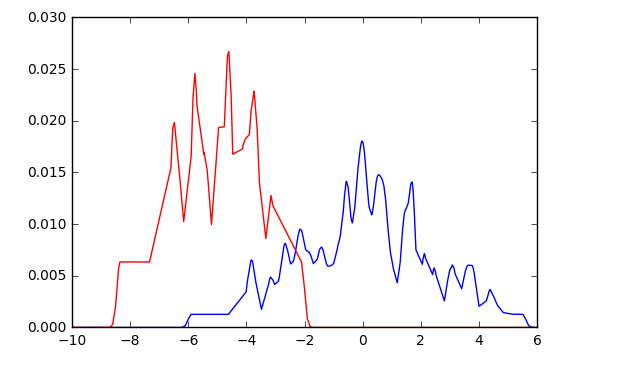
\includegraphics[scale=0.75]{1_a_1.png} \\
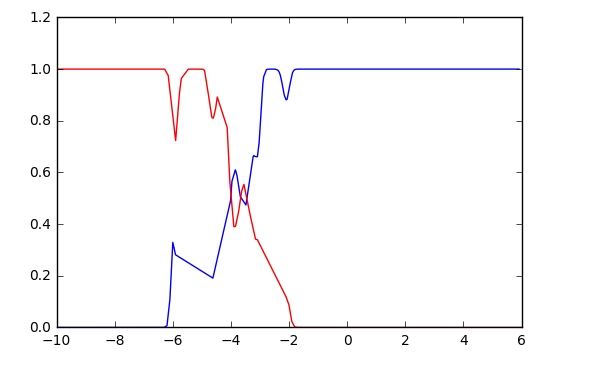
\includegraphics[scale=0.75]{1-a-2.png} \\
h=0.5 \\
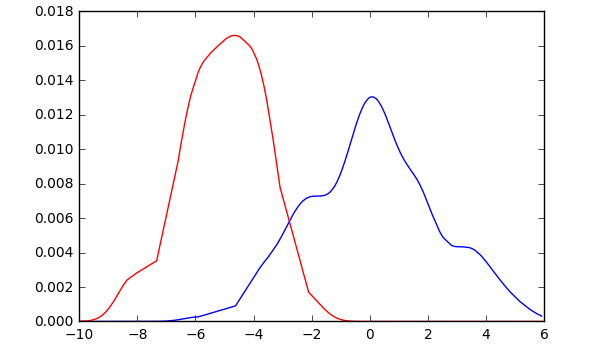
\includegraphics[scale=0.75]{1-a-3.png} \\
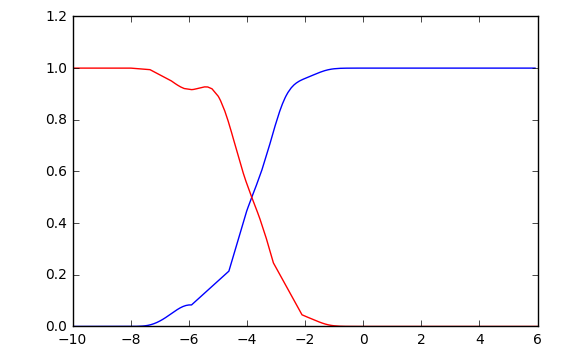
\includegraphics[scale=0.75]{1-a-4.png} \\
h=1 \\
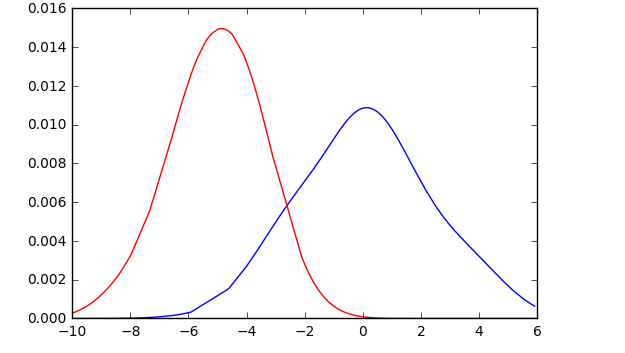
\includegraphics[scale=0.75]{1-a-6.png} \\
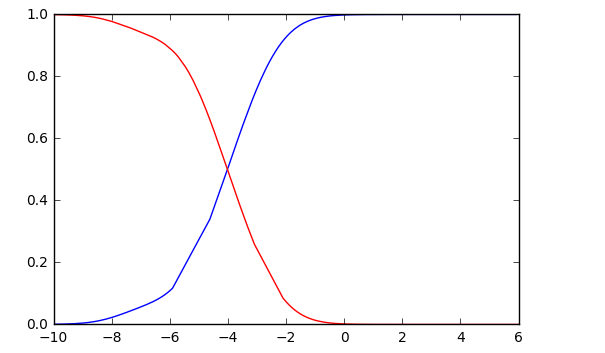
\includegraphics[scale=0.75]{1-a-7.png} \\
h=2 \\
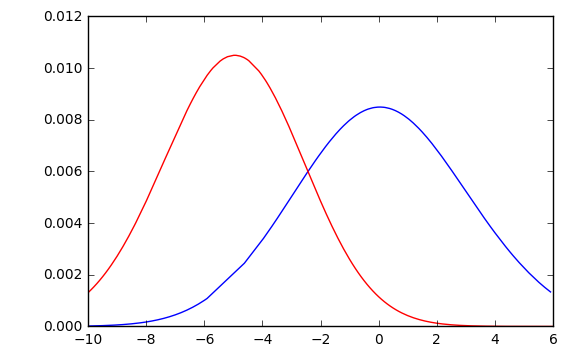
\includegraphics[scale=0.75]{1-a-8.png} \\
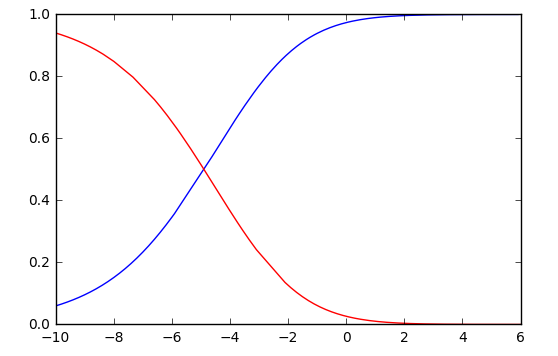
\includegraphics[scale=0.75]{1-a-9.png} \\


\subsection*{Q1-b}
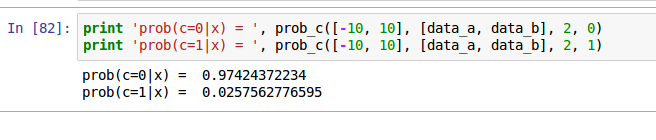
\includegraphics[scale=0.75]{1-b.png} \\
 
\subsection*{Q1-c}
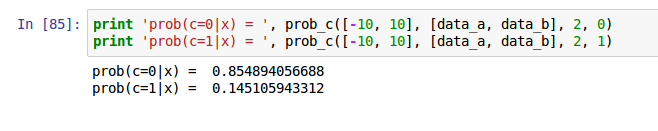
\includegraphics[scale=0.75]{1-c.png} \\


\section*{Q2}
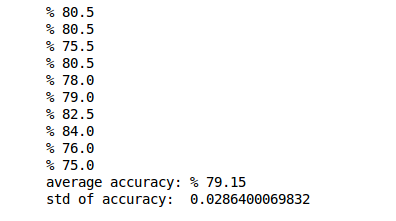
\includegraphics[scale=0.75]{2-1.png} \\
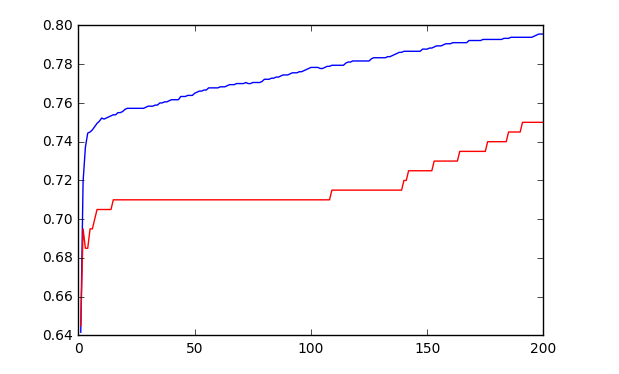
\includegraphics[scale=0.75]{2-2.png} \\

 
\end{document}